\subsection{Dataset and Data Preprocessing}

We use the Oxford-IIIT Pet Dataset for image classification. The dataset contains 37 categories of cats and dogs, with approximately 200 images per class. Following the official dataset split, the provided \texttt{trainval} subset is further divided into training and validation sets using stratified sampling with a validation ratio of 0.2, while the official \texttt{test} subset is used for final evaluation.

For training data, several data augmentation techniques are applied, including random resized cropping, random horizontal flipping, and color jittering. All images are normalized using the standard ImageNet mean and standard deviation. For validation and testing, deterministic preprocessing is adopted by resizing images to 256 pixels on the shorter side followed by center cropping to $224 \times 224$.

\begin{figure}[H]
    \centering
    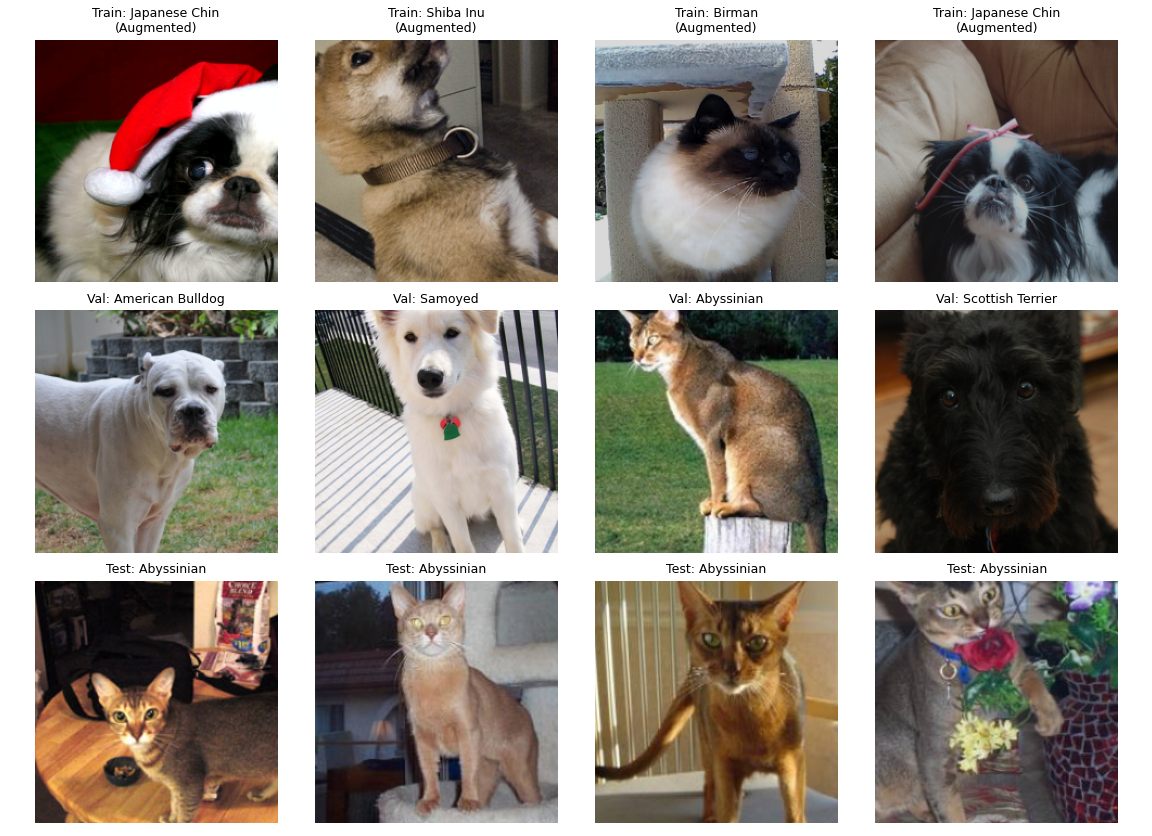
\includegraphics[width=0.85\textwidth]{figures/task1/data_visualization.png}
    \caption{Examples from the training, validation, and test sets. Training samples include random data augmentation.}
    \label{fig:data_visualization}
\end{figure}

In particular, we study the influence of the cropping scale used in \texttt{RandomResizedCrop}. Different lower bounds of the cropping ratio are tested, including $(0.08, 1.0)$, $(0.10, 1.0)$, and $(0.12, 1.0)$. Experimental results show that a smaller lower bound such as $(0.08, 1.0)$ produces overly strong augmentation and slows down convergence, while a larger lower bound such as $(0.12, 1.0)$ leads to earlier overfitting. The setting $(0.10, 1.0)$ achieves the best balance between convergence stability and generalization performance, and is therefore adopted in subsequent experiments.

\begin{figure}[H]
    \centering
    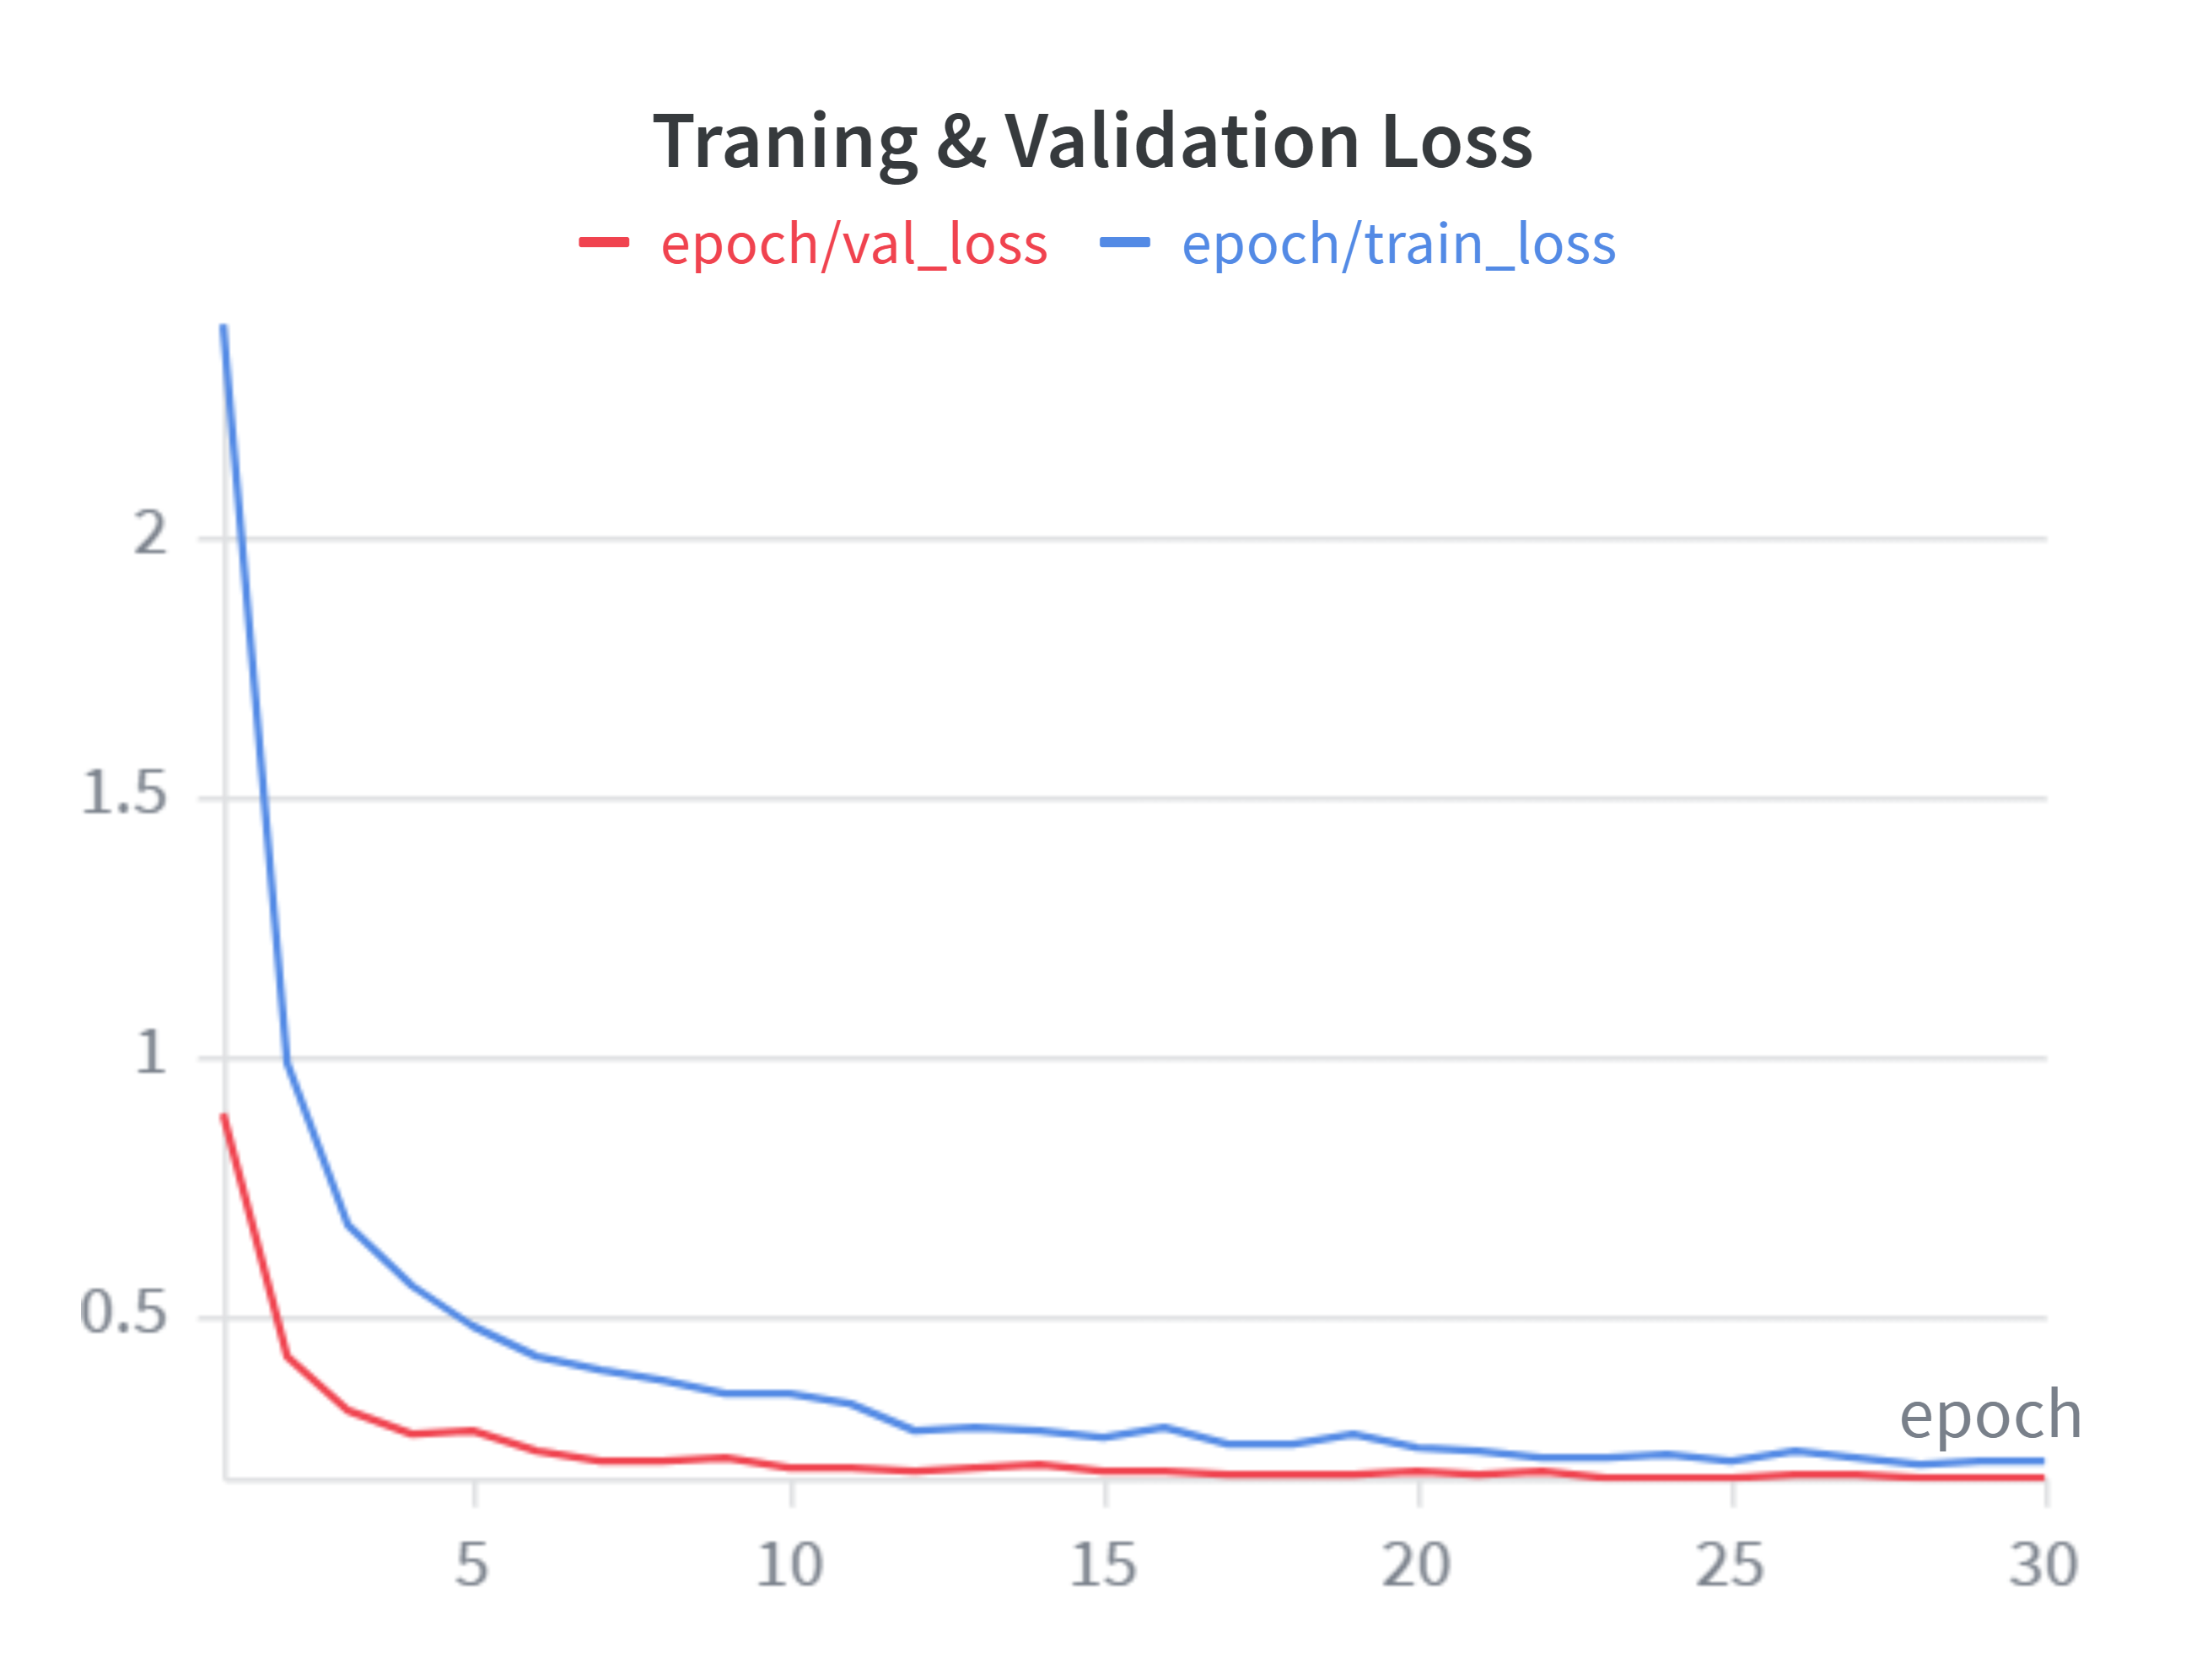
\includegraphics[width=0.32\textwidth]{figures/task1/aug_0.08_loss.png}
    \hfill
    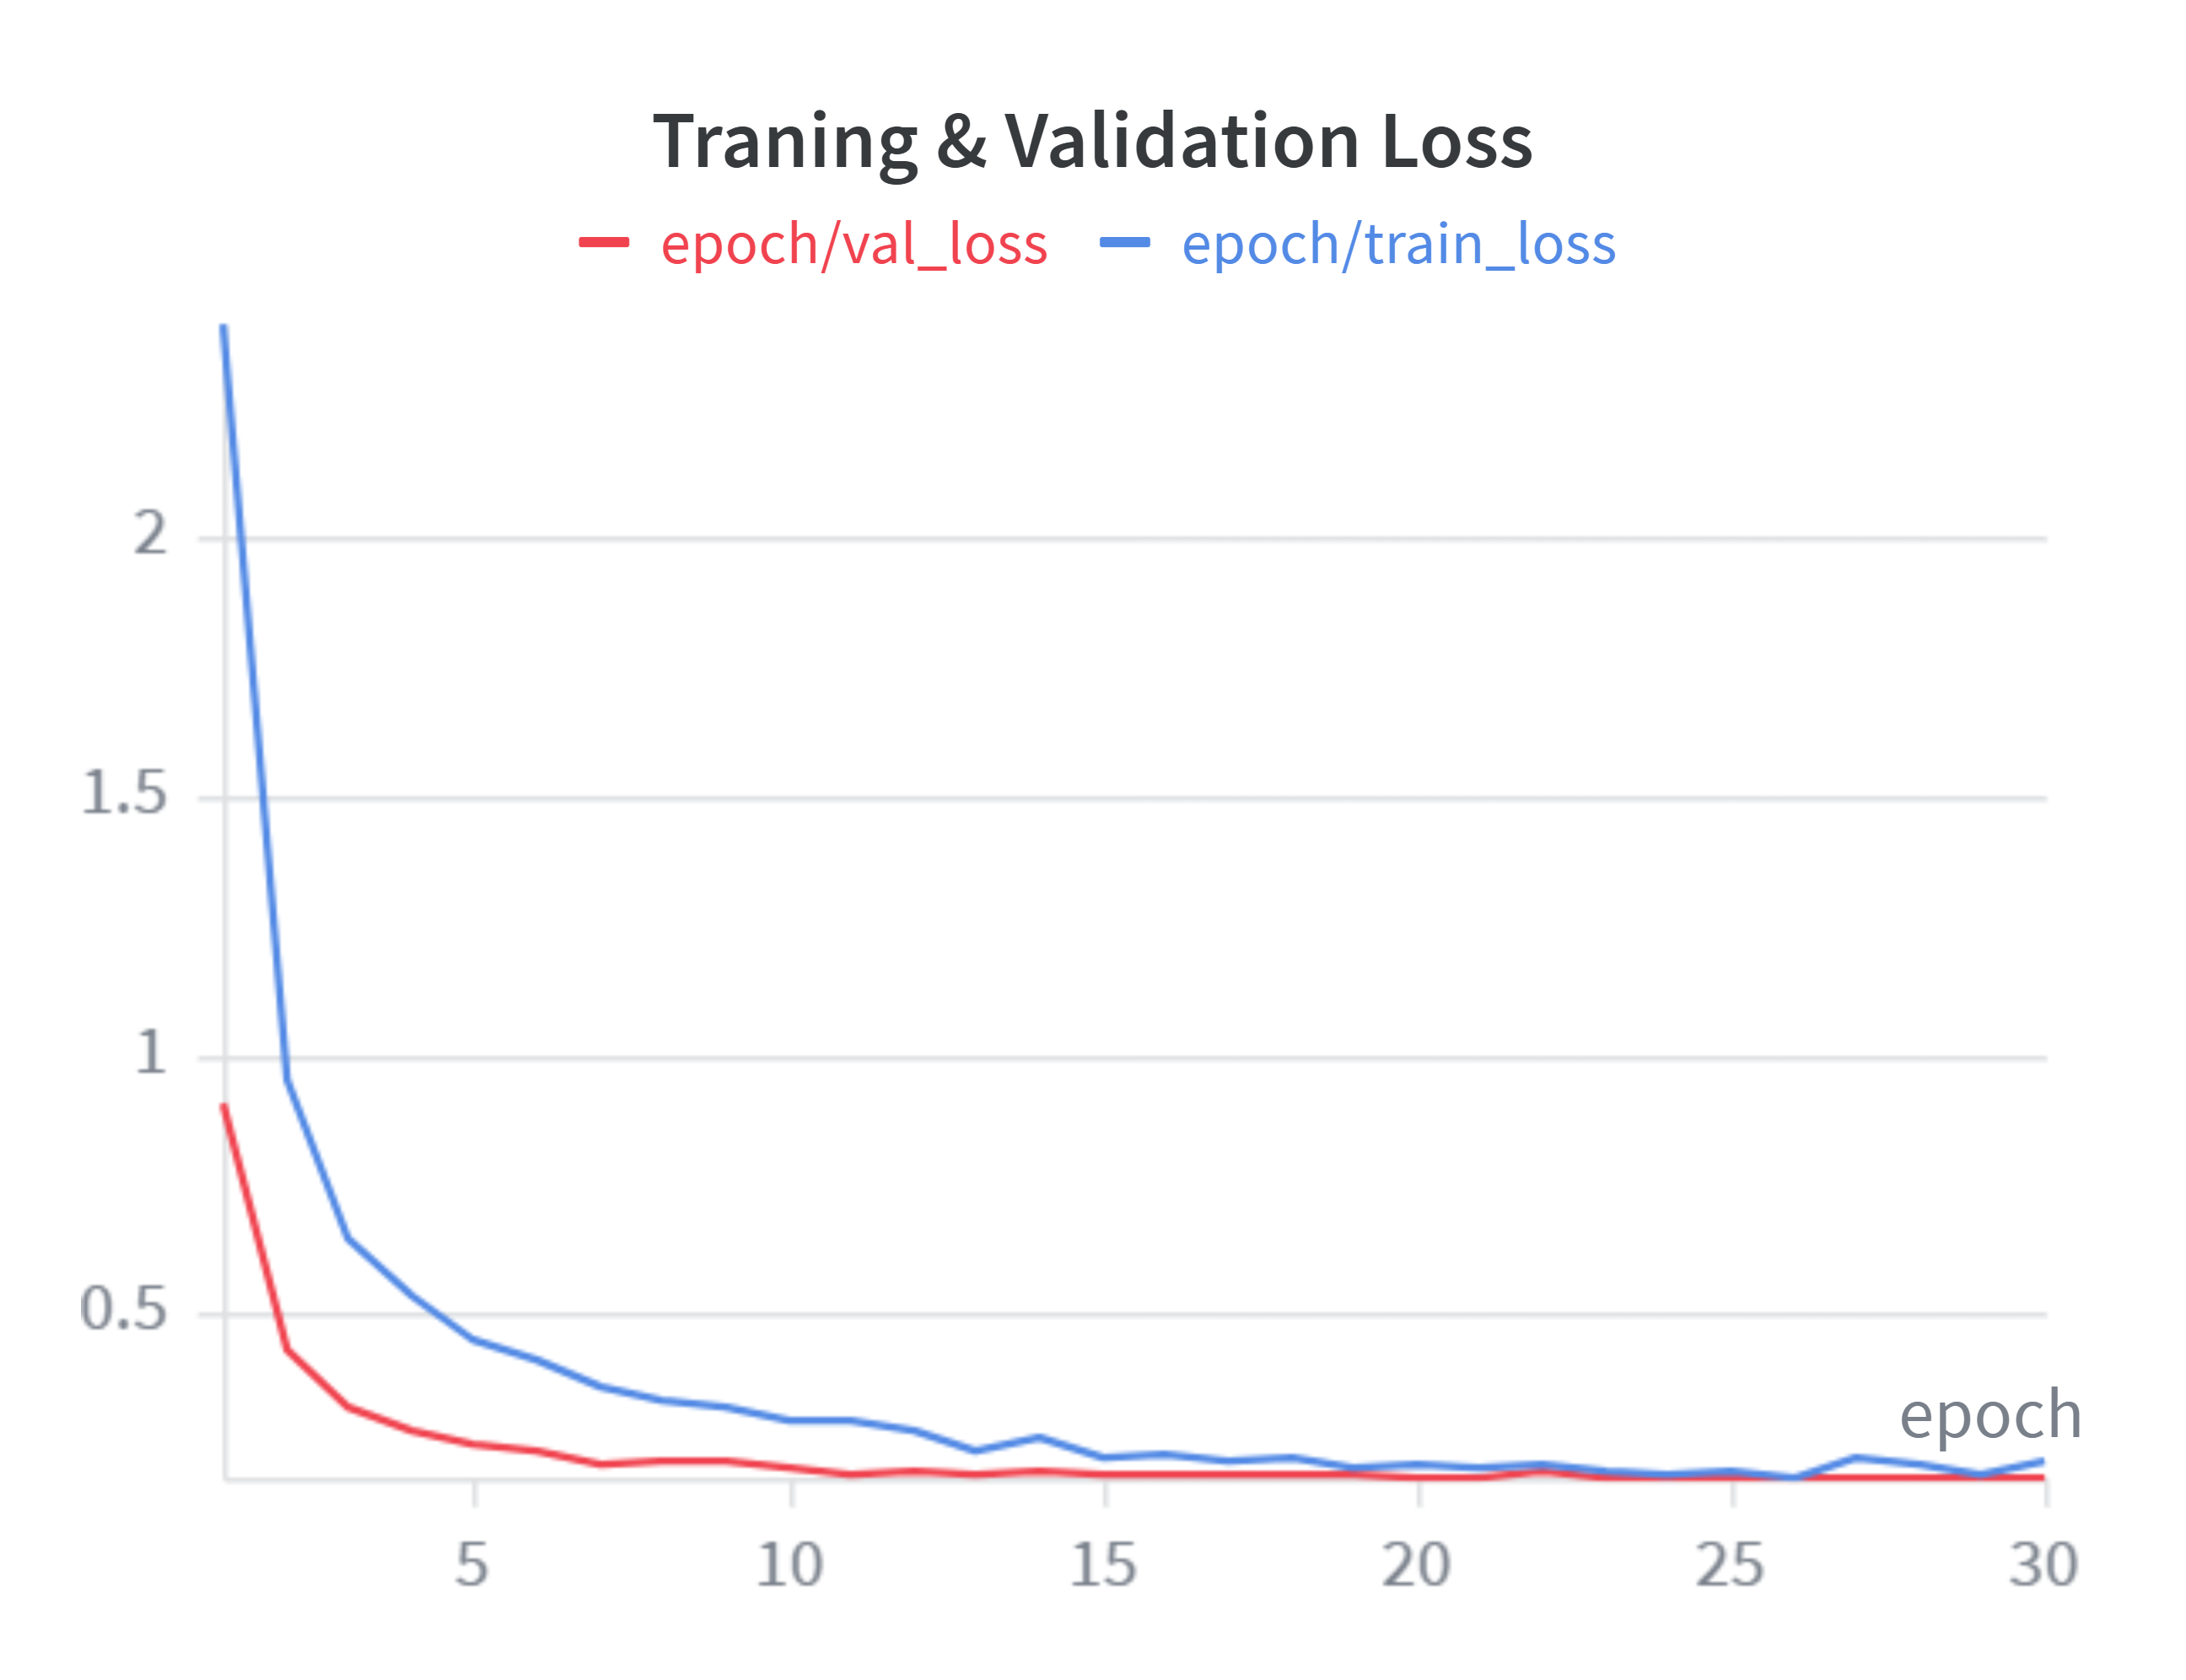
\includegraphics[width=0.32\textwidth]{figures/task1/aug_0.1_loss.png}
    \hfill
    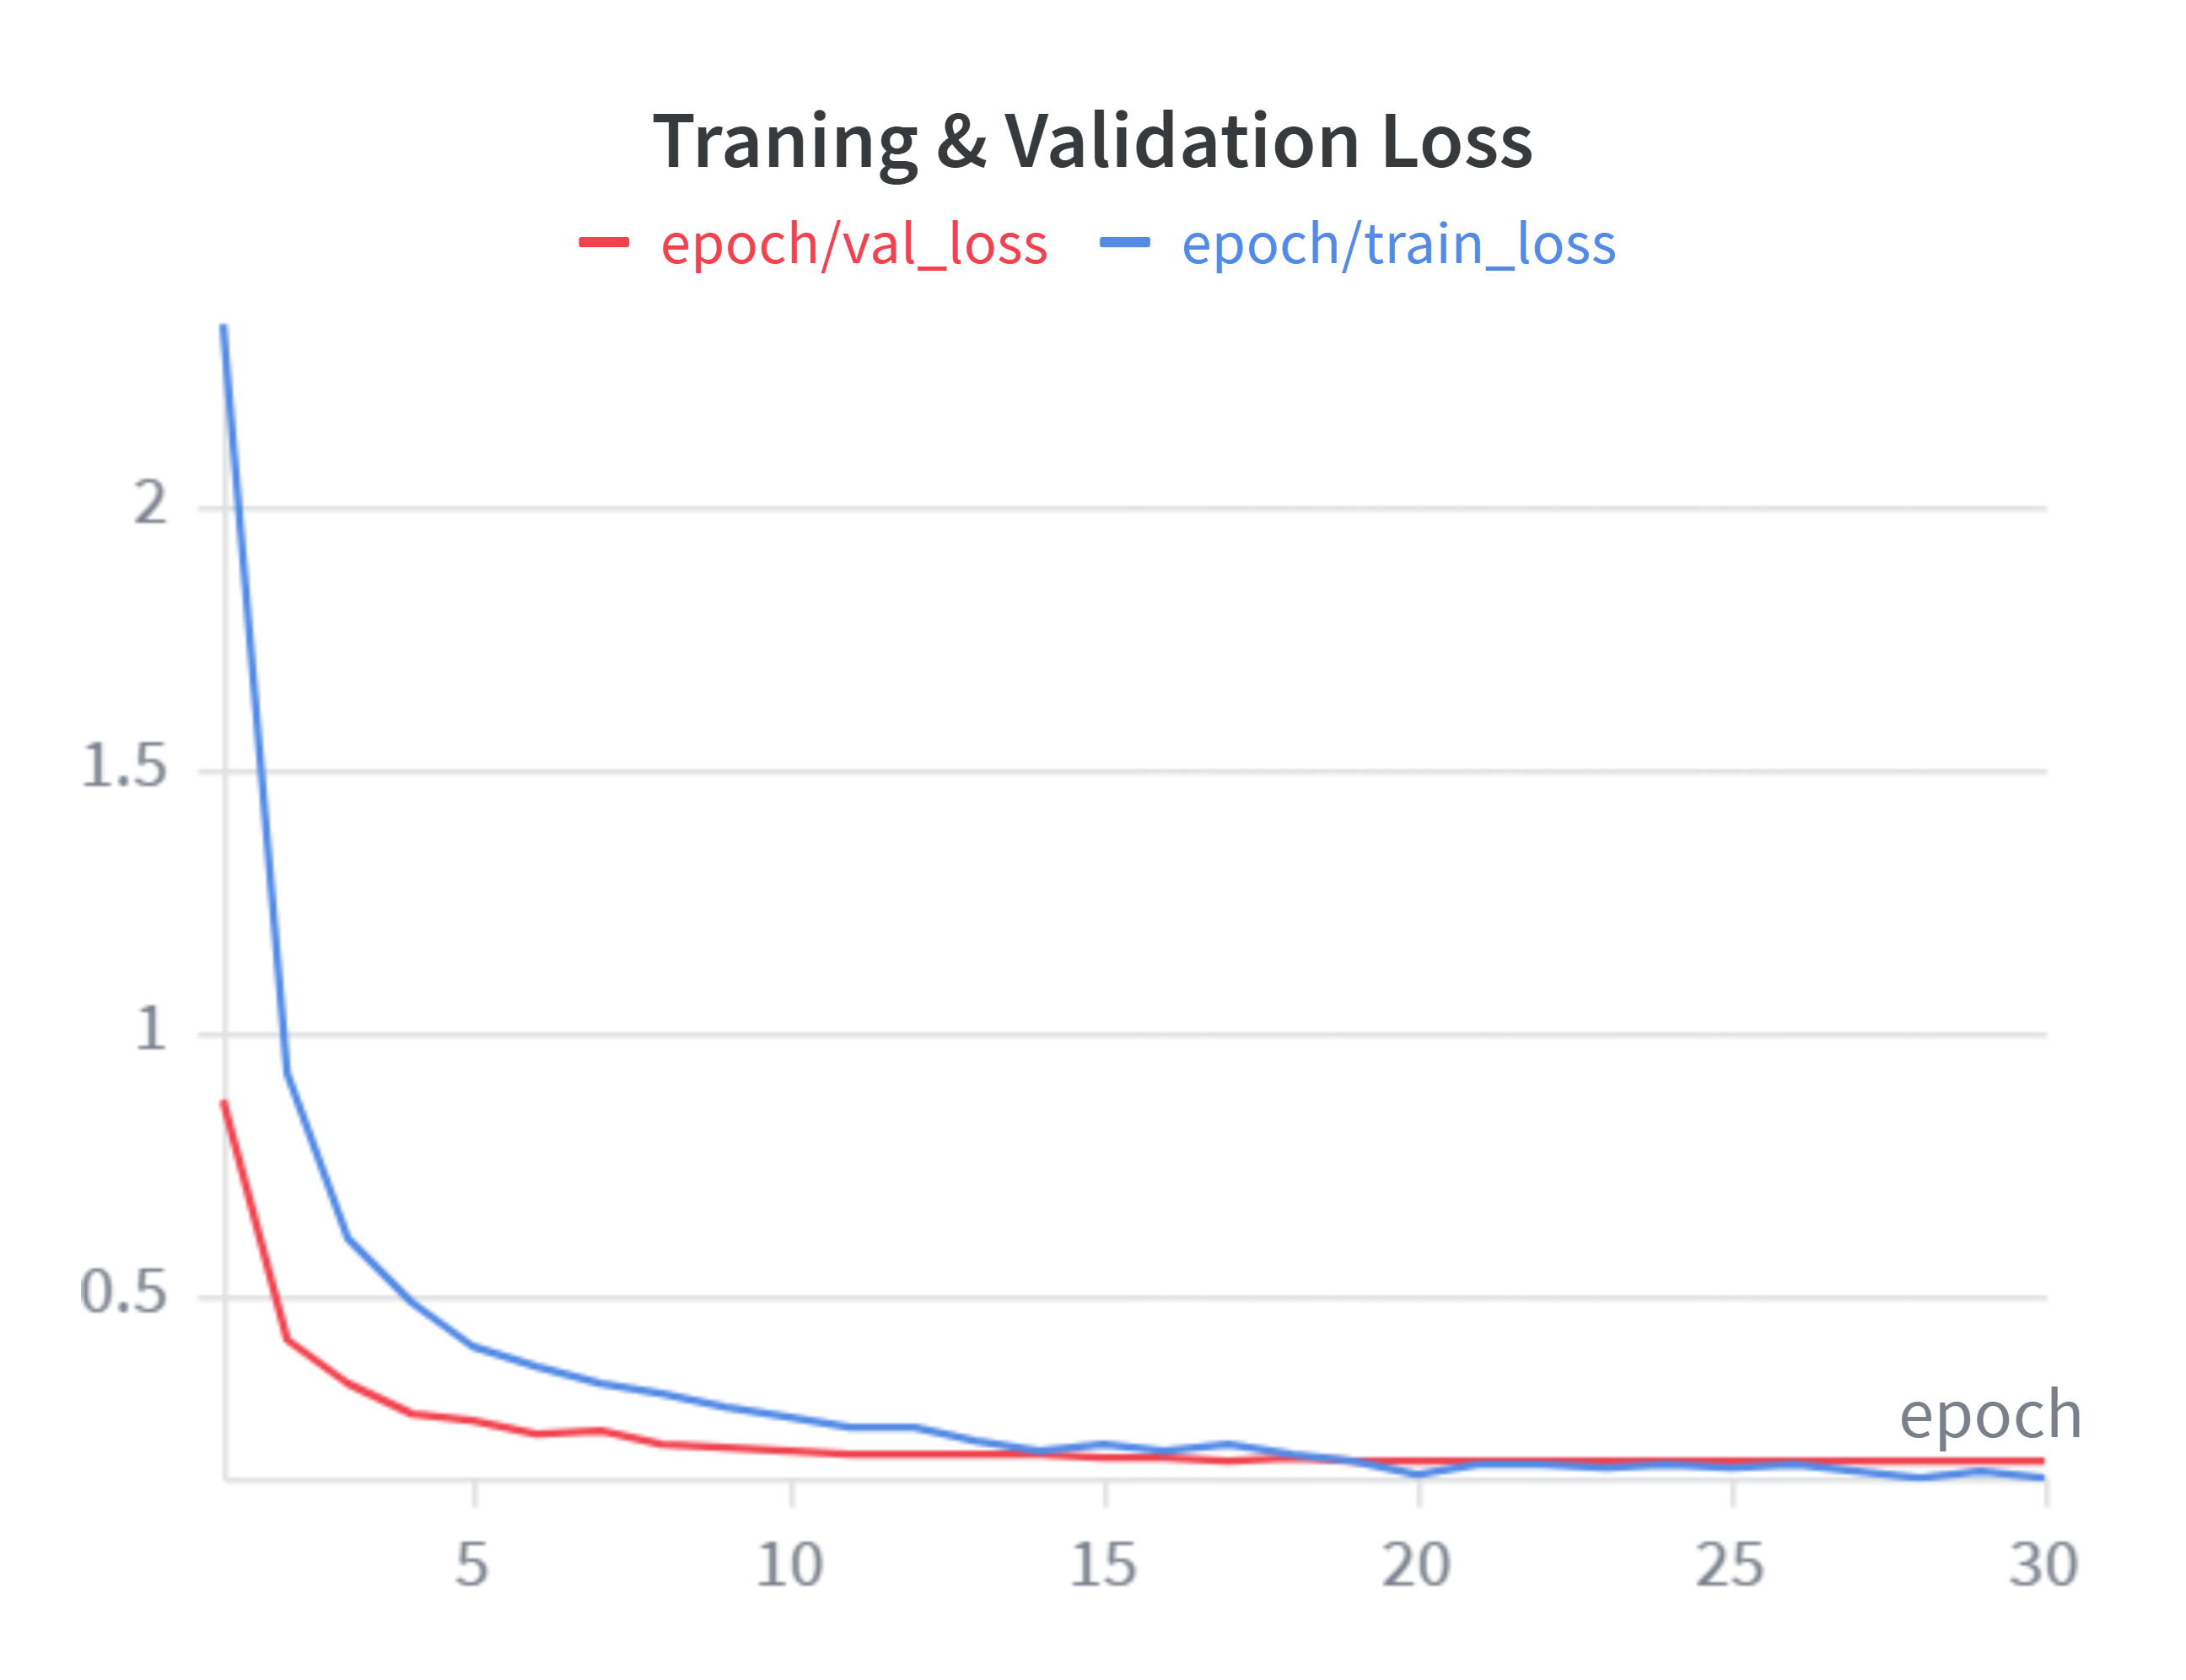
\includegraphics[width=0.32\textwidth]{figures/task1/aug_0.12_loss.png}
\caption{Training dynamics under different lower bounds of the cropping scale in \texttt{RandomResizedCrop}. From left to right, the lower bounds are 0.08, 0.10, and 0.12, respectively.}
    \label{fig:crop_scale_comparison}
\end{figure}
